%%%%%%%%%%%%%%%%%%%%%%%%%%%%%%%%%%%%%%%%%%%%%%%%%%%%%%%%%%%%%%%%%%%%%%%%%%%%%%%
%%
%% Copyright © 2022 Tropic Square s.r.o. (https://tropicsquare.com/)
%%
%% This work is subject to the license terms of the LICENSE.txt file in the
%% root directory of this source tree.
%%
%% If a copy of the LICENSE file was not distributed with this work, you can
%% obtain one at (https://tropicsquare.com/license).
%%
%%%%%%%%%%%%%%%%%%%%%%%%%%%%%%%%%%%%%%%%%%%%%%%%%%%%%%%%%%%%%%%%%%%%%%%%%%%%%%%
%
% LaTex class:
%    tropic_design_spec
%
%%%%%%%%%%%%%%%%%%%%%%%%%%%%%%%%%%%%%%%%%%%%%%%%%%%%%%%%%%%%%%%%%%%%%%%%%%%%%%%
%%%%%%%%%%%%%%%%%%%%%%%%%%%%%%%%%%%%%%%%%%%%%%%%%%%%%%%%%%%%%%%%%%%%%%%%%%%%%%%

% Specify Tropic Square document class
\documentclass[notconfidential]{tropic_design_spec}
\usepackage{textcomp}

\def\SCH{Secure Channel Handshake}
\def\SCS{Secure Channel Session}
\def\SCSN{Secure Channel Session Nonce}

\def\LLREQ{L2 Request frame}
\def\LLRSP{L2 Response frame}

\def\LLLCMD{L3 Command packet}
\def\LLLRES{L3 Result packet}

% Style of API Commands
\newcommand{\TsApiCmd}[1]{%
\mbox{\textit{\textbf{#1}}}%
}

% Style of protocol / command fields
\newcommand{\TsApiCmdFld}[1]{%
\mbox{\textbf{#1}}%
}


%%%%%%%%%%%%%%%%%%%%%%%%%%%%%%%%%%%%%%%%%%%%%%%%%%%%%%%%%%%%%%%%%%%%%%%%%%%%%%%
% Document properties and title page
%%%%%%%%%%%%%%%%%%%%%%%%%%%%%%%%%%%%%%%%%%%%%%%%%%%%%%%%%%%%%%%%%%%%%%%%%%%%%%%
\title{SPECT Firmware API}
\author{Vit Masek, Tropic Square}
\date{March 2024}

% Start of document
\begin{document}

% Parameters Needed by Design spec class (must be inside document)
% Set these parameters according to your project.
\def \projectname {SPECT Firmware}
\def \documentname {API Documentation}
\def \versionnumber {0.1}

% Title page
\maketitle


%%%%%%%%%%%%%%%%%%%%%%%%%%%%%%%%%%%%%%%%%%%%%%%%%%%%%%%%%%%%%%%%%%%%%%%%%%%%%%%
% Document revisions
% We revision with GIT, however, it does not mean that major changes in the
% document should not be kept also with document!
% In general, when you increase document version number, add also entry to
% this table with revisions saying what changed!
%%%%%%%%%%%%%%%%%%%%%%%%%%%%%%%%%%%%%%%%%%%%%%%%%%%%%%%%%%%%%%%%%%%%%%%%%%%%%%%
\section*{Version history}

\begin{TropicRatioLongTable4Col}
    {0.1}            {0.2}                  {0.2}           {0.5}
    {Version Tag     & Date                 & Author        &    Description                            }
     0.1             & 25.3.2024            & Vit Masek     &    Initial version (copy from
                                                                 TROPIC01 functional specification)     \Ttlb
\end{TropicRatioLongTable4Col}


%%%%%%%%%%%%%%%%%%%%%%%%%%%%%%%%%%%%%%%%%%%%%%%%%%%%%%%%%%%%%%%%%%%%%%%%%%%%%%%
% Table of contents
%%%%%%%%%%%%%%%%%%%%%%%%%%%%%%%%%%%%%%%%%%%%%%%%%%%%%%%%%%%%%%%%%%%%%%%%%%%%%%%
\pagebreak
\tableofcontents

%%%%%%%%%%%%%%%%%%%%%%%%%%%%%%%%%%%%%%%%%%%%%%%%%%%%%%%%%%%%%%%%%%%%%%%%%%%%%%%%%%%%%%%%%%%%%%%%%%%
%%%%%%%%%%%%%%%%%%%%%%%%%%%%%%%%%%%%%%%%%%%%%%%%%%%%%%%%%%%%%%%%%%%%%%%%%%%%%%%%%%%%%%%%%%%%%%%%%%%
% SPECT Operations
%%%%%%%%%%%%%%%%%%%%%%%%%%%%%%%%%%%%%%%%%%%%%%%%%%%%%%%%%%%%%%%%%%%%%%%%%%%%%%%%%%%%%%%%%%%%%%%%%%%
%%%%%%%%%%%%%%%%%%%%%%%%%%%%%%%%%%%%%%%%%%%%%%%%%%%%%%%%%%%%%%%%%%%%%%%%%%%%%%%%%%%%%%%%%%%%%%%%%%%

\pagebreak
\TsSection{SPECT Operations}

\newcommand{\SPECTCommandHead}[2]{
    \multicolumn{4}{|X}{\cellcolor{TropicBlue}\color{white}\textbf{#1}} &
    \multicolumn{1}{|>{\hsize=0.5\hsize}X}{\cellcolor{TropicBlue!70}\color{white}\Register{SPECT_OP_ID}:} &
    \multicolumn{1}{|>{\hsize=0.5\hsize}X|}{\cellcolor{TropicBlue!70}\color{white}#2} \\ \hline
}

\newcommand{\SPECTCommandDescription}[1]{
    \multicolumn{6}{|p{.9\textwidth}|}{#1} \\ \hline
}

\newcommand{\SPECTCommandMemHead}[1]{
    \rowcolor{gray!70}
    \multicolumn{6}{|c|}{\color{white}#1} \\ \hline
}

\newcommand{\SPECTCommandMem}[3]{
    \multicolumn{1}{|>{\hsize=0.2\hsize}X}{#1} &
    \multicolumn{1}{|>{\hsize=0.2\hsize}X}{#2} &
    \multicolumn{4}{|>{\hsize=1.5\hsize}X|}{#3} \\ \hline
}

\newcommand{\SPECTCommandCtx}[2]{
    \rowcolor{gray!70}
    \multicolumn{3}{|X}{\color{white}Context In} & \multicolumn{3}{|X|}{\color{white}Context Out} \\ \hline
    \multicolumn{3}{|X}{#1} & \multicolumn{3}{|X|}{#2} \\ \hline
}

\newcommand{\SPECTCommandTable}[1]{
    \begin{xltabular}{\textwidth}{|XXXXXX|}
    \hline
    #1
    \end{xltabular}
}


%%%%%%%%%%%%%%%%%%%%%%%%%%%%%%%%%%%%%%%%%%%%%%%%%%%%%%%%%%%%%%%%%%%%%%%%%%%%%%%%%%%%%%%%%%%%%%%%%%%%%%%%%%%%%%%%%%%%%
%%%%%%%%%%%%%%%%%%%%%%%%%%%%%%%%%%%%%%%%%%%%%%%%%%%%%%%%%%%%%%%%%%%%%%%%%%%%%%%%%%%%%%%%%%%%%%%%%%%%%%%%%%%%%%%%%%%%%

SPECT provides several operations for CPU that the CPU uses to perform more complex tasks, e. g. execute \LLLCMD{}s.

SPECT comes with two types of firmware:
\begin{itemize}
    \item \textbf{Boot FW} -- small firmware to support boot-up sequence of the chip.
    \item \textbf{Application FW} -- firmware that is preloaded into SPECTs instruction memory during
                                     boot-up sequence and used in final application.
\end{itemize}

\TropicNote{
    Besides these, another set of SPECT operations is available for debug purposes. These operations do not rely on
    the functionality of SCB, CPB nor KBUS. EDB can be set to debug mode.
}
\vspace{.3cm}

CPU specifies SPECT operation and SPECT firmware parameters by writing\linebreak
\Register{SPECT_CFG_WORD} on address 0x0100 of SPECTs address space (Data RAM In).

\vspace{.3cm}
\Register{SPECT_CFG_WORD}:

\begin{TropicRatioTable3Col}
    {0.5}                                 {0.25}                          {0.25}
    {[31:16]                            & [15:8]                        & [7:0]                  }
    \Register{SPECT_OP_DATA_IN_SIZE}    & \Register{SPECT_INOUT_SRC}    & \Register{SPECT_OP_ID} \Ttlb
\end{TropicRatioTable3Col}

CPU selects input data source via \Register{SPECT_INOUT_SRC[7:4]}.
\begin{itemize}
    \item \Register{SPECT_INOUT_SRC[7:4]}=0x0 -- SPECT operation takes input data from its Data RAM In.
    \item \Register{SPECT_INOUT_SRC[7:4]}=0x4 -- SPECT operation takes input data from Command Buffer.
\end{itemize}

CPU selects output data destination via \Register{SPECT_INOUT_SRC[3:0]}.
\begin{itemize}
    \item \Register{SPECT_INOUT_SRC[3:0]}=0x1 -- SPECT operation stores output data to its Data RAM Out.
    \item \Register{SPECT_INOUT_SRC[3:0]}=0x5 -- SPECT operation stores output data to Result Buffer.
\end{itemize}

CPU indicates number of bytes in Command Buffer or Data RAM In via \linebreak
\Register{SPECT_OP_DATA_IN_SIZE} field.

After SPECT finishes current operation, CPU reads \Register{SPECT_RES_WORD} from address \linebreak
0x1100 in SPECTs address space (Data RAM Out).

\pagebreak
\Register{SPECT_RES_WORD:}

\begin{TropicRatioTable3Col}
    {0.5}                                 {0.25}    {0.25}
    {[31:16]                            & [15:8]  & [7:0]                  }
    \Register{SPECT_OP_DATA_OUT_SIZE}   & --      & \Register{SPECT_OP_STATUS} \Ttlb
\end{TropicRatioTable3Col}

SPECT indicates status of the executed operation via \Register{SPECT_OP_STATUS}. SPECT also
indicates number of bytes in Data RAM Out or Result Buffer via \linebreak \Register{SPECT_OP_DATA_OUT_SIZE}.

\TropicNote{
    When SPECT executes operation that corresponds to one whole \LLLCMD{} (\LLLCMD{} is not
    split into multiple SPECT operations), then \Register{SPECT_OP_DATA_IN_SIZE} = \TsApiCmdFld{CMD_SIZE}
    and \Register{SPECT_OP_DATA_OUT_SIZE} = \TsApiCmdFld{RES_SIZE}.
}

\vspace{.3cm}
Values of \Register{SPECT_OP_STATUS} after SPECT operation execution can be following:

\hspace{.3cm}
\begin{TropicRatioTable2Col}
    {0.2}       {0.8}
    {Value      & Description}
    0x00        & SPECT Operation executed successfully     \Ttlb
    0xF1        & SPECT Context error                       \Ttlb
    0xF2        & SPECT KBUS error                          \Ttlb
    0xF3        & SPECT Invalid OP_ID error                 \Ttlb
    0xF4        & SPECT Invalid Curve Type error            \Ttlb
    0xF5        & SPECT GRV error                           \Ttlb
    0x11        & X25519 Error: invalid priv key            \Ttlb
    0x12        & X25519 Error: invalid pub key             \Ttlb
    0x21        & ECDSA Error: invalid ECDSA nonce ($k \equiv 0 \pmod{q_{P256}}$) \Ttlb
    0x22        & ECDSA Error: invalid ECDSA $r$ ($r \equiv 0 \pmod{q_{P256}}$)   \Ttlb
    0x23        & ECDSA Error: invalid ECDSA $s$ ($s \equiv 0 \pmod{q_{P256}}$)   \Ttlb
    0x24        & ECDSA Error: final verify fail            \Ttlb
    0x34        & EdDSA Error: invalid priv key $s$         \Ttlb
    0x35        & EdDSA Error: invalid pub key $A$          \Ttlb
    0x36        & EdDSA Error: final verify fail            \Ttlb
    0x41        & Point Integrity Error                     \Ttlb
\end{TropicRatioTable2Col}

To perform some more complex algorithm, such as EdDSA or secure channel establishment,
CPU needs to invoke SPECT multiple times. In such a case, SPECT keeps context between
execution of each partial operation.

SPECT Context is a set of values (e.g. keys or context of TMAC), that SPECT keeps inside
and uses them during its next operations. CPU shall invoke only such SPECT operation,
which input context matches the output context (or part of it) of previously invoked
SPECT operation. Otherwise the context would be corrupted or the result of such SPECT
operation undefined.

SPECT is capable of processing these \LLLCMD{}s by it self:
\begin{itemize}
    \item \TsApiCmd{ECC_Key_Generate} -- \textbf{ecc_key_generate} SPECT Op
    \item \TsApiCmd{ECC_Key_Store} -- \textbf{ecc_key_store} SPECT Op
    \item \TsApiCmd{ECC_Key_Read} -- \textbf{ecc_key_read} SPECT Op
    \item \TsApiCmd{ECC_Key_Erase} -- \textbf{ecc_key_erase} SPECT Op
    \item \TsApiCmd{ECDSA_Sign} -- \textbf{ecdsa_sign} SPECT Op
\end{itemize}

\TropicNote{
    \Register{SPECT_INOUT_SRC} is used for debug purpose, when unencrypted \LLLCMD{} is send to the device.
    That allows the CPU to bypass SCB and CPB and load the content of the \LLLCMD{} directly to SPECTs Data RAM In.
    In final implementation, no such bypass shall be possible.
}

%%%%%%%%%%%%%%%%%%%%%%%%%%%%%%%%%%%%%%%%%%%%%%%%%%%%%%%%%%%%%%%%%%%%%%%%%%%%%%%%%%%%%%%%%%%%%%%%%%%%%%%%%%%%%%%%%%%%%
%%%%%%%%%%%%%%%%%%%%%%%%%%%%%%%%%%%%%%%%%%%%%%%%%%%%%%%%%%%%%%%%%%%%%%%%%%%%%%%%%%%%%%%%%%%%%%%%%%%%%%%%%%%%%%%%%%%%%
% Application Firmware
%%%%%%%%%%%%%%%%%%%%%%%%%%%%%%%%%%%%%%%%%%%%%%%%%%%%%%%%%%%%%%%%%%%%%%%%%%%%%%%%%%%%%%%%%%%%%%%%%%%%%%%%%%%%%%%%%%%%%
%%%%%%%%%%%%%%%%%%%%%%%%%%%%%%%%%%%%%%%%%%%%%%%%%%%%%%%%%%%%%%%%%%%%%%%%%%%%%%%%%%%%%%%%%%%%%%%%%%%%%%%%%%%%%%%%%%%%%
\clearpage
\TsSubSection{SPECT Application Firmware}

%%%%%%%%%%%%%%%%%%%%%%%%%%%%%%%%%%%%%%%%%%%%%%%%%%%%%%%%%%%%%%%%%%%%%%%%%%%%%%%%%%%%%%%%%%%%%%%%%%%%%%%%%%%%%%%%%%%%%
% Control Commands
%%%%%%%%%%%%%%%%%%%%%%%%%%%%%%%%%%%%%%%%%%%%%%%%%%%%%%%%%%%%%%%%%%%%%%%%%%%%%%%%%%%%%%%%%%%%%%%%%%%%%%%%%%%%%%%%%%%%%
\subsubsection*{Control Operations}

\SPECTCommandTable{
    \SPECTCommandHead{clear}{0x00}

    \SPECTCommandDescription{Clears all GPRs and Data RAM In/Out. Clears context of SHA512 and TMAC.}
}

%%%%%%%%%%%%%%%%%%%%%%%%%%%%%%%%%%%%%%%%%%%%%%%%%%%%%%%%%%%%%%%%%%%%%%%%%%%%%%%%%%%%%%%%%%%%%%%%%%%%%%%%%%%%%%%%%%%%%
% ECC Key Operations
%%%%%%%%%%%%%%%%%%%%%%%%%%%%%%%%%%%%%%%%%%%%%%%%%%%%%%%%%%%%%%%%%%%%%%%%%%%%%%%%%%%%%%%%%%%%%%%%%%%%%%%%%%%%%%%%%%%%%
\subsubsection*{ECC Key Operations}

Following operations corresponds to eponymous \LLLCMD{}s. The value of each \Register{SPECT_OP_ID} is
equal to corresponding \LLLCMD{}s \TsApiCmdFld{CMD_ID}. The layout of inputs and outputs is also the same.

\SPECTCommandTable{
    \SPECTCommandHead{ecc_key_generate}{0x60}

    \SPECTCommandDescription{
        Computes ECC keys for ECDSA/EdDSA based on seed from TRNG, and stores them to user slot $i$ of
        ECC Key partition in Flash memory.
    }

    \SPECTCommandMemHead{Command Buffer / Data RAM In}
    \SPECTCommandMem{0x00}{1B}{\TsApiCmdFld{CMD_ID}}
    \SPECTCommandMem{0x01}{2B}{\TsApiCmdFld{SLOT} (Key slot $i$)}
    \SPECTCommandMem{0x03}{1B}{\TsApiCmdFld{CURVE} (Curve Type (P256 - ECDSA, Ed25519 - EdDSA))}

    \SPECTCommandMemHead{Result Buffer / Data RAM Out}
    \SPECTCommandMem{0x00}{1B}{\TsApiCmdFld{RESULT}}
}

\SPECTCommandTable{
    \SPECTCommandHead{ecc_key_store}{0x61}

    \SPECTCommandDescription{
        Computes ECC keys for ECDSA/EdDSA based on seed $k$, and stores them to user slot $i$ of
        ECC Key partition in Flash memory.
    }

    \SPECTCommandMemHead{Command Buffer / Data RAM In}
    \SPECTCommandMem{0x00}{1B}{\TsApiCmdFld{CMD_ID}}
    \SPECTCommandMem{0x01}{2B}{\TsApiCmdFld{SLOT} (Key slot $i$)}
    \SPECTCommandMem{0x03}{1B}{\TsApiCmdFld{CURVE} (Curve Type (P256 - ECDSA, Ed25519 - EdDSA))}
    \SPECTCommandMem{0x10}{32B}{\TsApiCmdFld{K} ($k$)}

    \SPECTCommandMemHead{Result Buffer / Data RAM Out}
    \SPECTCommandMem{0x00}{1B}{\TsApiCmdFld{RESULT}}
}

\pagebreak

\SPECTCommandTable{
    \SPECTCommandHead{ecc_key_read}{0x62}

    \SPECTCommandDescription{
        Reads ECDSA/EdDSA public key $A$ from slot $i$ of ECC Public Key partition.
    }

    \SPECTCommandMemHead{Command Buffer / Data RAM In}
    \SPECTCommandMem{0x00}{1B}{\TsApiCmdFld{CMD_ID}}
    \SPECTCommandMem{0x01}{2B}{\TsApiCmdFld{SLOT} (Key slot $i$)}

    \SPECTCommandMemHead{Result Buffer / Data RAM Out}
    \SPECTCommandMem{0x00}{1B}{\TsApiCmdFld{RESULT}}
    \SPECTCommandMem{0x01}{1B}{\TsApiCmdFld{CURVE} (Curve Type (P256, Ed25519))}
    \SPECTCommandMem{0x02}{1B}{\TsApiCmdFld{ORIGIN} (Identifier weather the key was stored or generated.)}
    \SPECTCommandMem{0x10}{64/32B}{\TsApiCmdFld{PUB_KEY} (ECDSA/EdDSA ECC Pub Key $A$)}
}

\SPECTCommandTable{
    \SPECTCommandHead{ecc_key_erase}{0x63}

    \SPECTCommandDescription{
        Erase ECDSA/EdDSA keys from slot $i$ of ECC Public/Private Key partition.
    }

    \SPECTCommandMemHead{Command Buffer / Data RAM In}
    \SPECTCommandMem{0x00}{1B}{\TsApiCmdFld{CMD_ID}}
    \SPECTCommandMem{0x01}{2B}{\TsApiCmdFld{SLOT} (Key slot $i$)}

    \SPECTCommandMemHead{Result Buffer / Data RAM Out}
    \SPECTCommandMem{0x00}{1B}{\TsApiCmdFld{RESULT}}
}

\pagebreak

%%%%%%%%%%%%%%%%%%%%%%%%%%%%%%%%%%%%%%%%%%%%%%%%%%%%%%%%%%%%%%%%%%%%%%%%%%%%%%%%%%%%%%%%%%%%%%%%%%%%%%%%%%%%%%%%%%%%%
% Secure Channel Handshake Operations
%%%%%%%%%%%%%%%%%%%%%%%%%%%%%%%%%%%%%%%%%%%%%%%%%%%%%%%%%%%%%%%%%%%%%%%%%%%%%%%%%%%%%%%%%%%%%%%%%%%%%%%%%%%%%%%%%%%%%
\subsubsection*{Secure Channel Handshake Operations}

All SPECT operations in this section are supported only with use of Data RAM In / Out
(\Register{SPECT_INOUT_SRC}=0x10).

\SPECTCommandTable{
    \SPECTCommandHead{x25519_kpair_gen}{0x11}

    \SPECTCommandDescription{
        Generates ephemeral X25519 key pair used during secure channel handshake.
    }

    \SPECTCommandMemHead{Data RAM Out}
    \SPECTCommandMem{0x1020}{32B}{$E_{TPUB}$}

    \SPECTCommandCtx{None}{\{$E_{TPRIV}$\}}
}

\SPECTCommandTable{
    \SPECTCommandHead{x25519_sc_et_eh}{0x12}

    \SPECTCommandDescription{
        Calculates $X1 =$ X25519($E_{TPRIV}$, $E_{HPUB}$).
    }

    \SPECTCommandMemHead{Data RAM In}
    \SPECTCommandMem{0x0020}{32B}{$E_{HPUB}$}

    \SPECTCommandMemHead{Data RAM Out}
    \SPECTCommandMem{0x1020}{32B}{$R1$}

    \SPECTCommandCtx{\{$E_{TPRIV}$\}}{\{$E_{TPRIV}$, $E_{HPUB}$\}}
}

\SPECTCommandTable{
    \SPECTCommandHead{x25519_sc_et_sh}{0x13}

    \SPECTCommandDescription{
        Calculates $R2 =$ X25519($E_{TPRIV}$, $S_{HIPUB}$).
    }

    \SPECTCommandMemHead{Data RAM In}
    \SPECTCommandMem{0x0020}{1B}{Key slot $i$}

    \SPECTCommandMemHead{Data RAM Out}
    \SPECTCommandMem{0x1020}{32B}{$R2$}

    \SPECTCommandCtx{\{$E_{TPRIV}$, $E_{HPUB}$\}}{\{$E_{HPUB}$\}}
}

\SPECTCommandTable{
    \SPECTCommandHead{x25519_sc_st_eh}{0x14}

    \SPECTCommandDescription{
        Calculates $R3 =$ X25519($S_{TPRIV}$, $E_{HPUB}$).
    }

    \SPECTCommandMemHead{Data RAM Out}
    \SPECTCommandMem{0x1020}{32B}{$R3$}

    \SPECTCommandCtx{\{$E_{HPUB}$\}}{None}
}

%%%%%%%%%%%%%%%%%%%%%%%%%%%%%%%%%%%%%%%%%%%%%%%%%%%%%%%%%%%%%%%%%%%%%%%%%%%%%%%%%%%%%%%%%%%%%%%%%%%%%%%%%%%%%%%%%%%%%
% EdDSA
%%%%%%%%%%%%%%%%%%%%%%%%%%%%%%%%%%%%%%%%%%%%%%%%%%%%%%%%%%%%%%%%%%%%%%%%%%%%%%%%%%%%%%%%%%%%%%%%%%%%%%%%%%%%%%%%%%%%%
\newpage
\subsubsection*{EdDSA Operations} \label{sec:spect_op:eddsa}

\SPECTCommandTable{
    \SPECTCommandHead{eddsa_set_context}{0x41}

    \SPECTCommandDescription{
        Sets context for Edwards Digital Signature Algorithm such as keys ($s, prefix, A$) and Secure Channel data ($SC_H$, $SC_N$).
    }

    \SPECTCommandMemHead{Command Buffer / Data RAM In}
    \SPECTCommandMem{0x01}{2B}{Key slot $i$}

    \SPECTCommandMemHead{Data RAM In}
    \SPECTCommandMem{0x00A0}{32B}{Secure Channel Hash $SC_H$}
    \SPECTCommandMem{0x00C0}{4B}{Secure Channel Nonce $SC_N$}

    \SPECTCommandCtx{None}{\{keys, $SC_N$, $SC_H$\}}
}

\SPECTCommandTable{
    \SPECTCommandHead{eddsa_nonce_init}{0x42}

    \SPECTCommandDescription{
        Initialize EdDSA nonce $r$ derivation -- TMAC_INIT($prefix$, 0x0C).
    }

    \SPECTCommandCtx{\{keys, $SC_N$, $SC_H$\}}{\{keys, TMAC ctx\}}
}

\SPECTCommandTable{
    \SPECTCommandHead{eddsa_nonce_update}{0x43}

    \SPECTCommandDescription{
        Processes next 144 bytes of decrypted message M. Updates TMAC context.
    }

    \SPECTCommandMemHead{Command Buffer / Data RAM In}
    \SPECTCommandMem{0x00}{144B}{Next 144 bytes of decrypted message M}


    \SPECTCommandCtx{\{keys, TMAC ctx\}}{\{keys, TMAC ctx\}}
}

\SPECTCommandTable{
    \SPECTCommandHead{eddsa_nonce_finish}{0x44}

    \SPECTCommandDescription{
        Finishes the EdDSA nonce derivation:\newline
        $r = $TMAC($prefix$, $SC_H$ || $SC_N$ || M, 0x0C) $\pmod{q_{Ed25519}}$.
    }

    \SPECTCommandMemHead{Command Buffer / Data RAM In}
    \SPECTCommandMem{0x00}{--}{Last up to 144 bytes of decrypted message M}

    \SPECTCommandCtx{\{keys, TMAC ctx, part of M\}}{\{keys, $r$, M size\}}
}
\pagebreak

\SPECTCommandTable{
    \SPECTCommandHead{eddsa_R_part}{0x45}

    \SPECTCommandDescription{
        Computes part $R$ of the signature -- $R = r \cdot G_{Ed25519}$.
    }

    \SPECTCommandCtx{\{keys, $r$, M size\}}{\{keys, $R$\}}
}

\SPECTCommandTable{
    \SPECTCommandHead{eddsa_e_at_once}{0x46}

    \SPECTCommandDescription{
        Computes $e$ at once in case of size of the message is less 64 bytes.
    }

    \SPECTCommandMemHead{Command Buffer / Data RAM In}
    \SPECTCommandMem{0x00}{--}{First up to 63 bytes of decrypted message M}

    \SPECTCommandCtx{\{keys, $R$\}}{\{keys, $R$, $e$\}}
}

\SPECTCommandTable{
    \SPECTCommandHead{eddsa_e_prep}{0x47}

    \SPECTCommandDescription{
        Prepares for derivation of $e$.
    }

    \SPECTCommandMemHead{Command Buffer / Data RAM In}
    \SPECTCommandMem{0x00}{64}{First 64 bytes of decrypted message M}

    \SPECTCommandCtx{\{keys, $R$\}}{\{keys, $R$, SHA512 ctx\}}
}

\SPECTCommandTable{
    \SPECTCommandHead{eddsa_e_update}{0x48}

    \SPECTCommandDescription{
        Processes next 128 bytes of decrypted message M. Updates SHA512 context.
    }

    \SPECTCommandMemHead{Command Buffer / Data RAM In}
    \SPECTCommandMem{0x00}{128B}{Next 128 bytes of decrypted message M}

    \SPECTCommandCtx{\{keys, $R$, SHA512 ctx\}}{\{keys, $R$, SHA512 ctx\}}
}

\SPECTCommandTable{
    \SPECTCommandHead{eddsa_e_finish}{0x49}

    \SPECTCommandDescription{
        Finishes derivation of $e = $SHA512($R$||$A$||M).
    }

    \SPECTCommandMemHead{Command Buffer / Data RAM In}
    \SPECTCommandMem{0x00}{--}{Last up to 128 bytes of decrypted message M}

    \SPECTCommandCtx{\{keys, $R$, SHA512 ctx\}}{\{keys, $R$, $e$\}}
}

\pagebreak

\SPECTCommandTable{
    \SPECTCommandHead{eddsa_finish}{0x4A}

    \SPECTCommandDescription{
        Computes second part $S$ of the signature -- $S = r + e \times s \pmod{q_{Ed25519}}$
    }

    \SPECTCommandMemHead{Result Buffer / Data RAM Out}
    \SPECTCommandMem{0x00}{1B}{\TsApiCmdFld{RESULT}}
    \SPECTCommandMem{0x10}{64B}{Signature (\TsApiCmdFld{R}, \TsApiCmdFld{S})}

    \SPECTCommandCtx{\{keys, $R$, $e$\}}{None}
}

%%%%%%%%%%%%%%%%%%%%%%%%%%%%%%%%%%%%%%%%%%%%%%%%%%%%%%%%%%%%%%%%%%%%%%%%%%%%%%%%%%%%%%%%%%%%%%%%%%%%%%%%%%%%%%%%%%%%%
% ECDSA
%%%%%%%%%%%%%%%%%%%%%%%%%%%%%%%%%%%%%%%%%%%%%%%%%%%%%%%%%%%%%%%%%%%%%%%%%%%%%%%%%%%%%%%%%%%%%%%%%%%%%%%%%%%%%%%%%%%%%
\subsubsection*{ECDSA Operations}

\SPECTCommandTable{
    \SPECTCommandHead{ecdsa_sign}{0x70}

    \SPECTCommandDescription{
        Generate ECDSA signature ($r, s$) of a message digest $z$ using ECC keys from slot $i$.
    }

    \SPECTCommandMemHead{Command Buffer / Data RAM In}

    \SPECTCommandMem{0x01}{2B}{\TsApiCmdFld{SLOT} (ECC Key slot $i$)}
    \SPECTCommandMem{0x10}{32B}{\TsApiCmdFld{MSG_HASH} (Message digest $z$)}

    \SPECTCommandMemHead{Data RAM In}
    \SPECTCommandMem{0x00A0}{32B}{Secure Channel Hash $SCh$}
    \SPECTCommandMem{0x00C0}{4B}{Secure Channel Nonce $SCn$}

    \SPECTCommandMemHead{Result Buffer / Data RAM Out}
    \SPECTCommandMem{0x0}{1B}{\TsApiCmdFld{RESULT} (Command Result)}
    \SPECTCommandMem{0x10}{64B}{Signature (\TsApiCmdFld{R}, \TsApiCmdFld{S})}
}

\TropicNote{
    eddsa_set_context and ecdsa_sign SPECT operation takes Secure Channel Handshake Hash ($SCh$) and
    Secure Channel Session Nonce ($SCn$) always from Data RAM In, never from Command Buffer regardless
    of the \Register{SPECT_INOUT_SRC} value.
}

%%%%%%%%%%%%%%%%%%%%%%%%%%%%%%%%%%%%%%%%%%%%%%%%%%%%%%%%%%%%%%%%%%%%%%%%%%%%%%%%%%%%%%%%%%%%%%%%%%%%%%%%%%%%%%%%%%%%%
% Boot Firmware
%%%%%%%%%%%%%%%%%%%%%%%%%%%%%%%%%%%%%%%%%%%%%%%%%%%%%%%%%%%%%%%%%%%%%%%%%%%%%%%%%%%%%%%%%%%%%%%%%%%%%%%%%%%%%%%%%%%%%
\newpage
\TsSubSection{SPECT Boot Firmware}

%%%%%%%%%%%%%%%%%%%%%%%%%%%%%%%%%%%%%%%%%%%%%%%%%%%%%%%%%%%%%%%%%%%%%%%%%%%%%%%%%%%%%%%%%%%%%%%%%%%%%%%%%%%%%%%%%%%%%
% SHA512
%%%%%%%%%%%%%%%%%%%%%%%%%%%%%%%%%%%%%%%%%%%%%%%%%%%%%%%%%%%%%%%%%%%%%%%%%%%%%%%%%%%%%%%%%%%%%%%%%%%%%%%%%%%%%%%%%%%%%

\subsubsection*{EdDSA Verify}
\SPECTCommandTable{
    \SPECTCommandHead{eddsa_verify}{0x4B}

    \SPECTCommandDescription{
        Verifies a EdDSA signature of 32-byte message $M$ using public key $A$.
    }

    \SPECTCommandMemHead{Data RAM In}
    \SPECTCommandMem{0x0020}{64B}{Signature (\TsApiCmdFld{R}, \TsApiCmdFld{S})}
    \SPECTCommandMem{0x0060}{32B}{Public key $A$}
    \SPECTCommandMem{0x0080}{32B}{Message $M$}

    \SPECTCommandMemHead{Data RAM Out}
    \SPECTCommandMem{0x0000}{4B}{Result: 0x0B5E55ED $\Rightarrow$ verified, else failed}
    \SPECTCommandMem{0x0004}{4B}{Result: 0xBA11FADE $\Rightarrow$ verified, else failed}
}

\subsubsection*{SHA512 Operations}

\textcolor{red}{Removed since SPECT FW v0.3.0}

\SPECTCommandTable{
    \SPECTCommandHead{sha512_init}{0x51}

    \SPECTCommandDescription{
        Initialize SHA512 unit.
    }

    \SPECTCommandCtx{None}{SHA512 ctx}
}

\textcolor{red}{Removed since SPECT FW v0.3.0}

\SPECTCommandTable{
    \SPECTCommandHead{sha512_update}{0x52}

    \SPECTCommandDescription{
        Process one 128B block of data with SHA512.
    }

    \SPECTCommandMemHead{Data RAM In}
    \SPECTCommandMem{0x10}{128B}{Data}

    \SPECTCommandCtx{SHA512 ctx}{SHA512 ctx}
}

\textcolor{red}{Removed since SPECT FW v0.3.0}

\SPECTCommandTable{
    \SPECTCommandHead{sha512_final}{0x53}

    \SPECTCommandDescription{
        Process last 128B block of data that contains SHA512 padding.
    }

    \SPECTCommandMemHead{Data RAM In}
    \SPECTCommandMem{0x10}{128B}{Data}

    \SPECTCommandMemHead{Data RAM Out}
    \SPECTCommandMem{0x10}{64B}{Digest}

    \SPECTCommandCtx{SHA512 ctx}{None}
}

\pagebreak

\subsubsection*{SHA512 example:}

Let \textbf{M} be a 326 byte data (\texttt{u8 M [326]}). SHA512(\textbf{M}) is computed as follows:

\begin{enumerate}
    \item Pad the data with SHA512 padding to multiple of 128B, see \ref{fig.sha512_padding}.
    \item Initialize SPECTs SHA512 unit with \textbf{sha512_init()}.
    \item Process first chunk with \textbf{sha512_update(M[0:127])}.
    \item Process second chunk with \textbf{sha512_update(M[128:255])}.
    \item Process the rest of \textbf{M} with \textbf{sha512_final(M[256:383])}.
    \item Data RAM Out now contains the SHA512 digest of \textbf{M}.
\end{enumerate}

\begin{figure}[h]
    \centering%
    \includegraphics[width=.9\textwidth]{%
        \detokenize{img/FS_SHA512_PADDING.pdf}%
    }
    \caption{SHA512 Padding}%
    \label{fig.sha512_padding}%
\end{figure}

%%%%%%%%%%%%%%%%%%%%%%%%%%%%%%%%%%%%%%%%%%%%%%%%%%%%%%%%%%%%%%%%%%%%%%%%%%%%%%%%%%%%%%%%%%%%%%%%%%%%%%%%%%%%%%%%%%%%%
% Debug
%%%%%%%%%%%%%%%%%%%%%%%%%%%%%%%%%%%%%%%%%%%%%%%%%%%%%%%%%%%%%%%%%%%%%%%%%%%%%%%%%%%%%%%%%%%%%%%%%%%%%%%%%%%%%%%%%%%%%
\newpage
\TsSubSection{SPECT Debug Operations}

All SPECT operations in this section are supported only with use of Data RAM In / Out
(\Register{SPECT_INOUT_SRC}=0x01).

\SPECTCommandTable{
    \SPECTCommandHead{x25519_dbg}{0x9F}

    \SPECTCommandDescription{
        Performs general X25519 algorithm. $R = $ X25519($Priv$, $Pub$)
    }

    \SPECTCommandMemHead{Data RAM In}
    \SPECTCommandMem{0x0020}{32B}{Private key $Priv$}
    \SPECTCommandMem{0x0040}{32B}{Public key $Pub$}

    \SPECTCommandMemHead{Data RAM Out}
    \SPECTCommandMem{0x1020}{32B}{Result $R$}
}

\SPECTCommandTable{
    \SPECTCommandHead{ecdsa_sign_dbg}{0xAF}

    \SPECTCommandDescription{
        Computes signature of message digest $z$ using ECDSA.
    }

    \SPECTCommandMemHead{Data RAM In}
    \SPECTCommandMem{0x0010}{32B}{Message digest $z$}

    \SPECTCommandMem{0x0040}{64B}{Private key pair ($d$, $w$)}
    \SPECTCommandMem{0x00A0}{32B}{Secure Channel Hash $SC_H$}
    \SPECTCommandMem{0x00C0}{ 4B}{Secure Channel Nonce $SC_N$}
    \SPECTCommandMem{0x0160}{64B}{Public key ($A_x, A_y$)}

    \SPECTCommandMemHead{Data RAM Out}
    \SPECTCommandMem{0x1010}{64B}{Signature}
}

\SPECTCommandTable{
    \SPECTCommandHead{eddsa_set_context_dbg}{0xBF}

    \SPECTCommandDescription{
        Sets context for EdDSA sequence from Data RAM In only.
    }

    \SPECTCommandMemHead{Data RAM In}
    \SPECTCommandMem{0x0040}{64B}{Private keys ($s$, $prefix$)}
    \SPECTCommandMem{0x00A0}{32B}{Secure Channel Hash $SC_H$}
    \SPECTCommandMem{0x00C0}{ 4B}{Secure Channel Nonce $SC_N$}
    \SPECTCommandMem{0x0300}{32B}{Public key $A$}

    \SPECTCommandCtx{None}{\{keys, $SC_N$, $SC_H$\}}
}

\newpage
\TsSubSection{Processing \LLLCMD{} using SPECT}

CPU always issues first 16 byte chunk of \LLLCMD{}s \Register{CMD_CIPHERTEXT} to SCB. SCB decrypts
the chunk and passes it to CPB. CPB checks user access privileges and stores the decrypted
\Register{CMD_CIPHERTEXT} into Command Buffer. Then CPU reads the \LLLCMD{}s \TsApiCmdFld{CMD_ID}
from CPB. Following three cases may occur:

\subsubsection*{\TsApiCmdFld{CMD_ID} corresponds to one of \TsApiCmd{ECC_Key_*}}

In this case, CPU issues the rest of \Register{CMD_CIPHERTEXT} to SCB. After that, Command Buffer
contains all data and information needed for execution of the corresponding \linebreak SPECT
operation. CPU sets \Register{SPECT_INOUT_SRC}=0x45 and invokes SPECT.

SPECT reads Command Buffer and performs the corresponding SPECT operation. Then it stores all output
data for the \LLLRES{} to Result Buffer, sets \linebreak \Register{SPECT_OP_DATA_OUT_SIZE} to number
of bytes it has stored and notifies CPU.

CPU reads \Register{SPECT_OP_DATA_OUT_SIZE} bytes from Result Buffer, that are encrypted by SCB
resulting in \Register{RES_CIPHERTEXT} of the \LLLRES{}.

\subsubsection*{\TsApiCmdFld{CMD_ID} corresponds to \TsApiCmd{ECDSA_Sign}}

In this case, the process is almost the same as in the case of \TsApiCmd{ECC_Key_*}. In addition, CPU reads
the Secure Channel Nonce and Secure Channel Hash from SCB and loads it in to SPECTs Data RAM In before
invoking SPECT.

\subsubsection*{\TsApiCmdFld{CMD_ID} corresponds to \TsApiCmd{EDDSA_Sign}}

In this case, the \LLLCMD{} has arbitrary length, depending on the length of the \TsApiCmdFld{MSG} field.
Therefore the \TsApiCmd{EDDSA_Sign} \LLLCMD{} is processed with a sequence of SPECT operations from
\ref{sec:spect_op:eddsa}. We can divide this sequence into 5 phases:

\begin{enumerate}
    \item Setting context and loading keys -- \textbf{eddsa_set_context} / \textbf{eddsa_set_context_dbg}
    \item Computing nonce $r$ using TMAC -- \textbf{eddsa_nonce_*}
    \item Computing signature part \TsApiCmdFld{R} -- \textbf{eddsa_R_part}
    \item Computing e = SHA512(\TsApiCmdFld{R}, $A$, \TsApiCmdFld{MSG}) -- \textbf{eddsa_e_*}
    \item Computing signature part \TsApiCmdFld{S} -- \textbf{eddsa_finish}
\end{enumerate}

Figures \ref{EdDSA_DF} shows the sequence in detail.

\pagebreak

\begin{figure}[H]
    \centering
    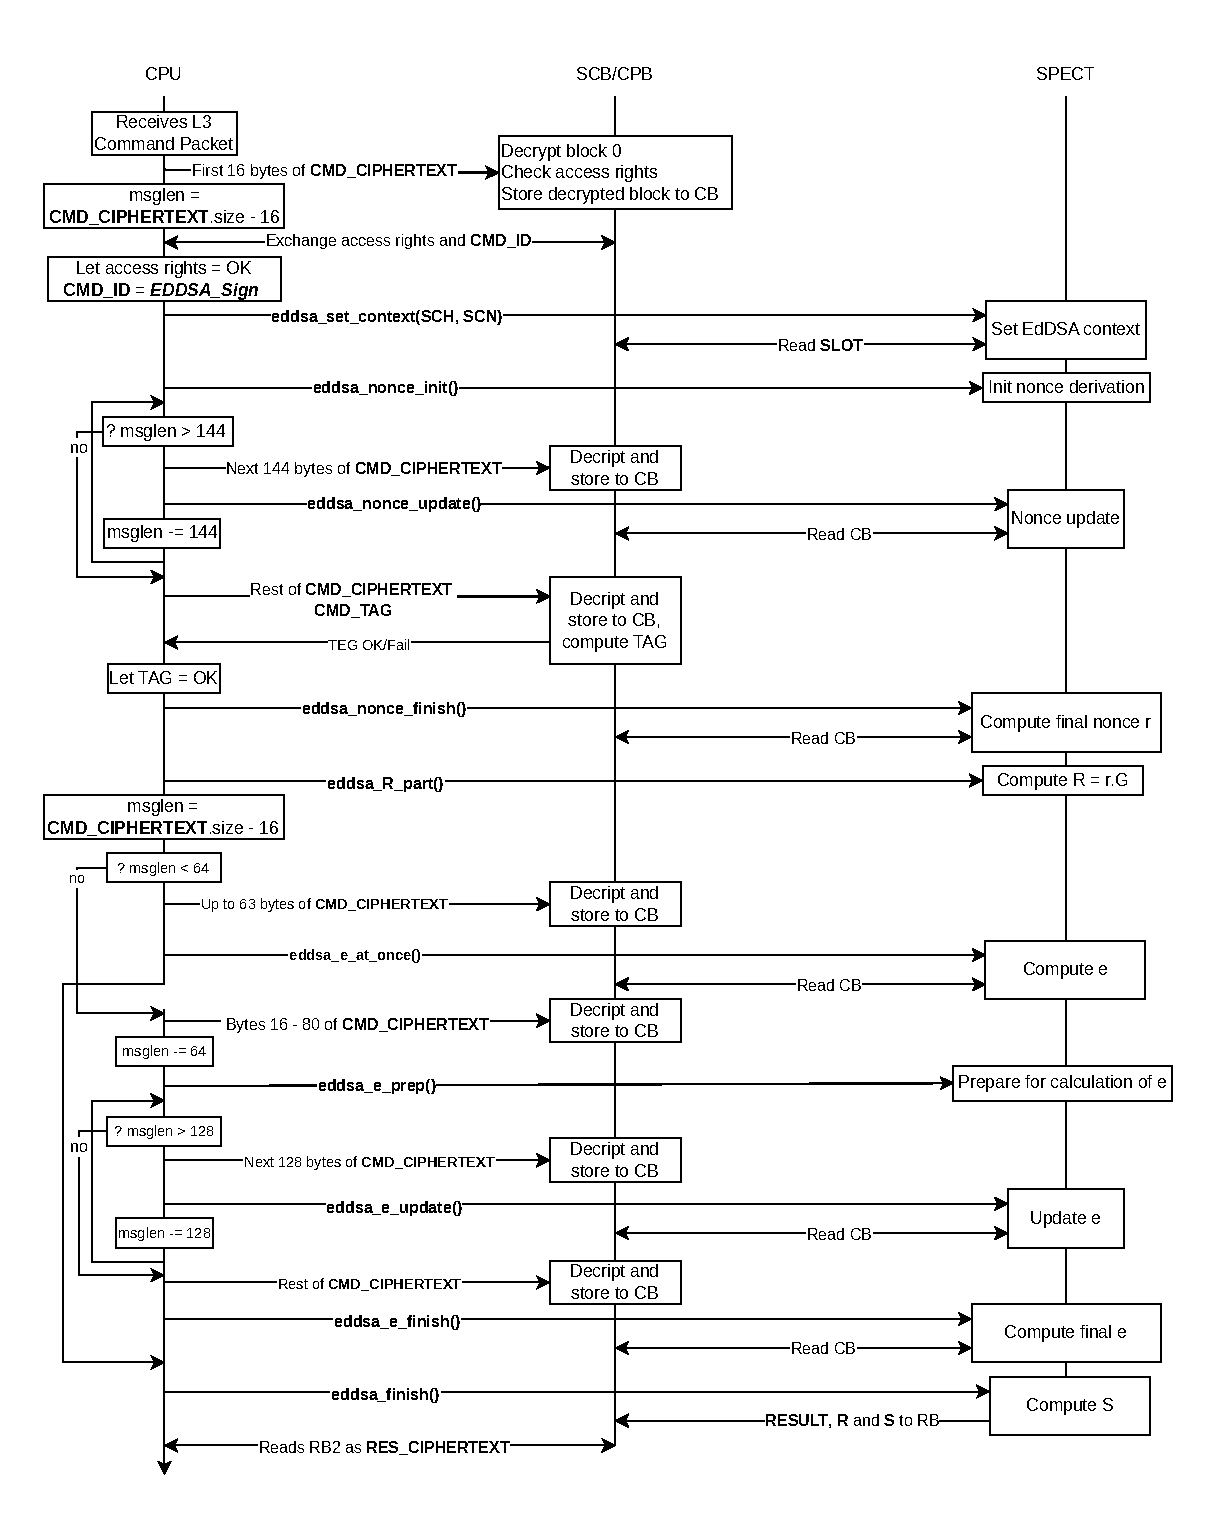
\includegraphics[width=\textwidth]{%
        \detokenize{img/FS_EDDSA_DF.pdf}%
    }
    \caption{\projectname\space - EDDSA Data Flow }
    \label{EdDSA_DF}
\end{figure}

%%%%%%%%%%%%%%%%%%%%%%%%%%%%%%%%%%%%%%%%%%%%%%%%%%%%%%%%%%%%%%%%%%%%%%%%%%%%%%%
% Open issues
%%%%%%%%%%%%%%%%%%%%%%%%%%%%%%%%%%%%%%%%%%%%%%%%%%%%%%%%%%%%%%%%%%%%%%%%%%%%%%%
\TsSection{Open Issues}

\PrintOpenIssueSummary

\end{document}
